\documentclass[10pt,a4paper]{article}

\usepackage[utf8]{inputenc}
\usepackage[margin=1in]{geometry}
\usepackage{graphicx}
\usepackage{booktabs}
\usepackage{amsmath,amssymb,bm}
\usepackage{caption}
\usepackage{subcaption}
\usepackage[hidelinks]{hyperref}
\usepackage{authblk}

\captionsetup{font=small,labelfont=bf}
\setlength{\parskip}{2pt}

\title{\vspace{-1.5em}Do Skip Connections and Graph Rewiring Complement Each Other?\\
A Controlled Study of Information Propagation in GNNs}
\author{Anonymous submission}
\date{}

\begin{document}
\maketitle
\vspace{-2.5em}

\begin{center}
\small Code: \url{https://anonymous.4open.science/r/grl-miniproject} \quad(anonymised)
\end{center}
\vspace{0.5em}

\begin{abstract}
\noindent
Oversmoothing and over-squashing are two opposing failures of \emph{information
propagation} in graph neural networks (GNNs): the former destroys signal by
\emph{too much} mixing at depth, the latter by \emph{too little} signal surviving
a topological bottleneck. Two popular remedies target them separately---residual
(skip) connections for oversmoothing and graph rewiring for over-squashing. We ask
whether these remedies \emph{complement} each other or whether fixing one failure
mode aggravates the other. Using two controlled synthetic testbeds (a stochastic
block model for oversmoothing, a barbell signal-propagation task for over-squashing)
and a $2\times2$ design over \{plain, skip\}$\times$\{original, rewired\}, evaluated
across five seeds, we find a clear \emph{asymmetric} trade-off: curvature-based
rewiring reliably fixes over-squashing but \emph{worsens} oversmoothing, while skip
connections mitigate oversmoothing and moderate over-squashing but fail on severe
bottlenecks. Only the combination is robust on both axes. We support the mechanism
with Jacobian-sensitivity and Ollivier--Ricci curvature analyses, and give a critical
account of where the design is fragile.
\end{abstract}

\section{Introduction}
\label{sec:intro}

Message-passing GNNs propagate information by repeatedly aggregating neighbour
features. This single mechanism underlies two well-documented and \emph{opposite}
pathologies of \emph{information propagation}. \textbf{Oversmoothing}: as depth
grows, repeated averaging drives all node representations toward a common
vector, so deeper networks become less, not more, discriminative
\cite{li2018deeper,oono2020,rusch2023survey}. \textbf{Over-squashing}: when a task
requires information to travel through a structural bottleneck, an exponentially
growing receptive field is compressed into a fixed-width vector and long-range
signal is lost \cite{alon2021,topping2022,digiovanni2023}.

Two remedies are usually studied in isolation. \emph{Skip (residual) connections}
\cite{he2016,xu2018jk} add a node's previous-layer representation back at each
layer, preserving identity and counteracting oversmoothing. \emph{Graph rewiring}
\cite{topping2022} alters the input topology to relieve bottlenecks; Stochastic
Discrete Ricci Flow (SDRF) adds edges at the most negatively curved (bottleneck)
locations. Because the two pathologies are opposites, a natural and---to our
knowledge---underexamined question is whether the two fixes interfere.

\paragraph{Research question (a).}
\emph{Do residual connections and graph rewiring complement each other in
addressing the oversmoothing/over-squashing trade-off, or does fixing one failure
mode worsen the other?} This matters because practitioners routinely combine
architectural and topological tricks; if they interact adversarially, ``stacking
fixes'' can silently hurt. We study it in a deliberately small, controlled setting
where the ground-truth difficulty of each pathology is known by construction.

\section{Methods}
\label{sec:methods}

\paragraph{Approach and goals (b).}
We isolate each pathology in a synthetic graph where its severity is a controllable
knob, and cross two factors in a $2\times2$ grid: model
$\in\{\text{GCN},\text{SkipGCN}\}$ and topology $\in\{\text{original},\text{rewired}\}$,
giving \textsc{GCN}, \textsc{SkipGCN}, \textsc{GCN+Rewire}, \textsc{Skip+Rewire}.
The goal is not peak accuracy but to read off \emph{which intervention helps or
hurts which pathology}, and to confirm the mechanism with propagation diagnostics.

\paragraph{Models (c).}
Both models stack $K$ \texttt{GCNConv} layers (hidden width $64$, ReLU, dropout
$0.3$). \textsc{SkipGCN} uses the Practical-3 residual update
$\bm{H}^{(t)}=\mathrm{ReLU}\big(\mathrm{GCNConv}(\bm{H}^{(t-1)})\big)+
\mathrm{proj}(\bm{H}^{(t-1)})$, where $\mathrm{proj}$ is a linear map when widths
differ and identity otherwise.

\paragraph{Graph A: oversmoothing (SBM).}
A stochastic block model with $4$ communities of $50$ nodes ($p_{\text{intra}}{=}0.7$,
$p_{\text{inter}}{=}0.02$, $16$ random Gaussian features); node task = community.
Dense intra-community wiring makes repeated averaging collapse representations.

\paragraph{Graph B: over-squashing (barbell).}
Two $5$-cliques joined by a bridge of length $b$ (Fig.~\ref{fig:topology}). A binary
signal is planted at a \emph{source} node in the left clique; all other nodes carry
only noise. The model must predict the signal \emph{only} at a \emph{target} node in
the right clique, so the answer must cross the bridge (distance $1{+}b$ hops). Loss
and accuracy are read at the target node, preventing any pooling shortcut. We sweep
depth $K$ and bridge length $b$ independently. We use $400$ graphs per setting,
$60/20/20$ split.

\paragraph{Rewiring.}
We use an \emph{SDRF-inspired} rewiring: each step targets the most negatively
curved edge (Ollivier--Ricci, $\alpha{=}0$) and adds a shortcut between its
low-degree neighbours. This differs from \cite{topping2022} in the edge-selection
rule (deterministic, degree-based, rather than softmax-sampled by curvature
improvement); we therefore label it ``SDRF-inspired''. Fig.~\ref{fig:topology}
shows it removes the negative-curvature bridge edges and collapses the source--target
distance.

\paragraph{Diagnostics.}
We quantify \emph{oversmoothing} with mean average distance
(MAD, mean pairwise cosine distance of embeddings) and Dirichlet energy
\cite{li2018deeper,rusch2023survey}, and \emph{over-squashing} with the Jacobian
sensitivity $\lVert\partial \bm h_v/\partial \bm x_u\rVert$ as a function of the
$u$--$v$ graph distance \cite{topping2022,digiovanni2023}.

\paragraph{Protocol and assumptions (c).}
Adam; SBM trained full-batch ($\text{lr}=0.01$), barbell mini-batched
($\text{lr}=0.005$, batch $32$); early stopping (patience $20$/$30$) on a validation
split. \textbf{Every accuracy/diagnostic is averaged over 5 seeds and reported as
mean\,$\pm$\,std.} For the SBM the graph is fixed and seeds vary initialisation; for
the barbell each seed re-draws the dataset and re-initialises. Key assumptions: the
synthetic graphs faithfully isolate each pathology, and MAD/Jacobian are valid
proxies for smoothing/squashing.

\begin{figure}[t]
\centering
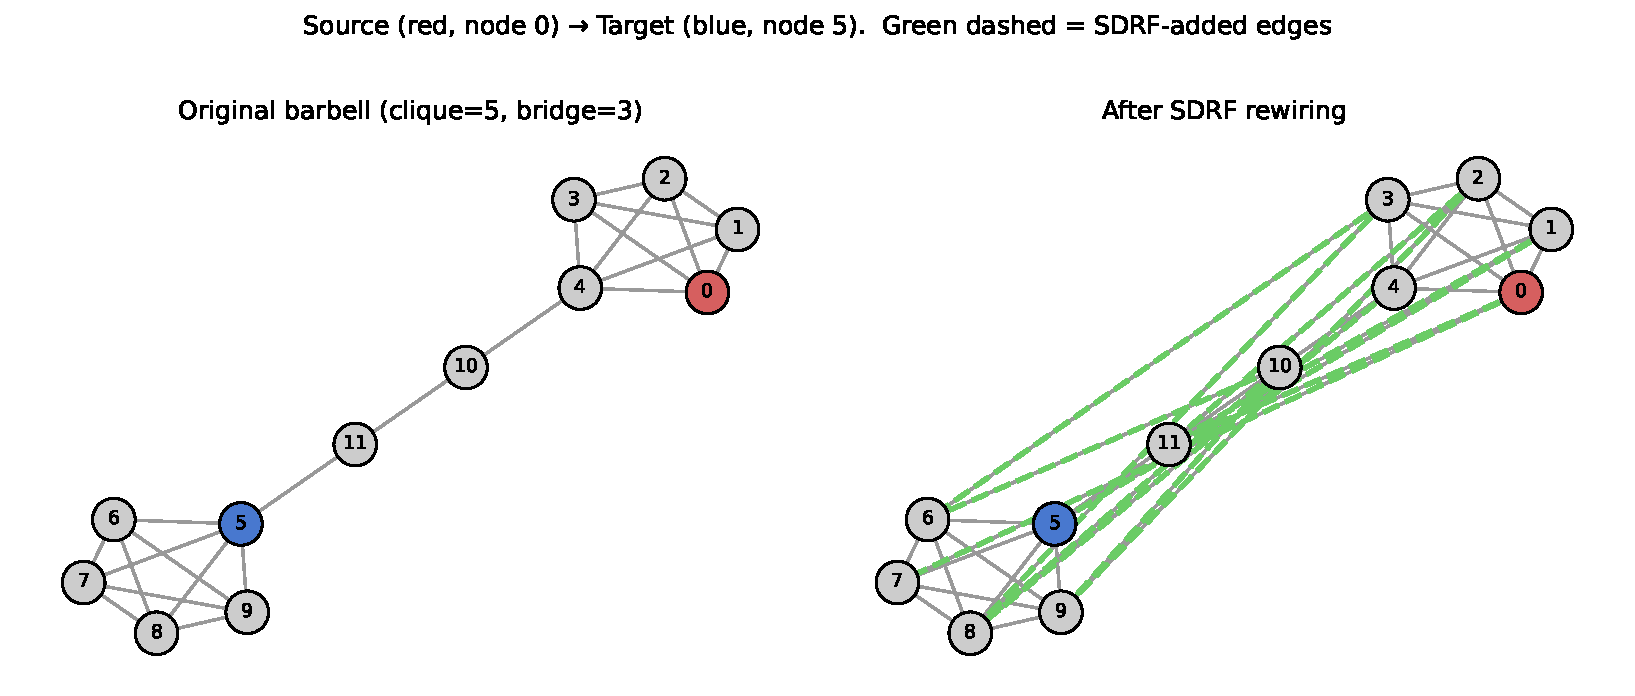
\includegraphics[width=0.86\linewidth]{barbell_topology.pdf}
\caption{Barbell task before/after SDRF-inspired rewiring. Source (red) and target
(blue) are separated by a thin bridge of negative curvature; rewiring (green dashed
edges) connects the cliques directly, collapsing the diameter from $5$ to $2$.}
\label{fig:topology}
\end{figure}

\section{Results}
\label{sec:results}

\paragraph{Rewiring removes the bottleneck (sanity).}
The barbell has exactly $4/23$ negatively curved edges---the bridge---and SDRF
eliminates them, shifting the whole curvature distribution positive
(App.~\ref{app:curv}). This confirms the intervention does what it should before we
read its effect on learning.

\paragraph{Experiment A---oversmoothing (Fig.~\ref{fig:expA}).}
Plain GCN collapses with depth: accuracy $1.0\!\to\!0.19\pm.03$ at $K{=}16$ and
MAD $\to 0.000\pm.000$ (every seed fully collapses). Skip connections substantially
\emph{mitigate} this (Acc $0.97\pm.03$ at $K{=}8$) but do \emph{not} fully solve it:
at $K{=}16$ they are $0.86\pm.26$---high variance, i.e.\ some initialisations still
fail. Crucially, \textbf{rewiring worsens oversmoothing}: \textsc{GCN+Rewire}
($0.44\pm.15$ at $K{=}8$) is below \textsc{GCN} ($0.64\pm.23$), with lower MAD,
because added edges accelerate mixing.

\paragraph{Experiment B---over-squashing (Fig.~\ref{fig:expB}, Table~\ref{tab:bridge}).}
With depth (bridge $b{=}3$, $4$ hops needed), GCN never reliably solves the task at
any $K$ (e.g.\ $0.57\pm.22$ at $K{=}8$), whereas \textsc{SkipGCN} is perfect for
$K\ge8$ ($1.000\pm.000$). Sweeping bridge length at $K{=}8$ gives the headline
result: \textbf{rewiring solves every bridge length} ($1.000\pm.000$ throughout),
while skip connections degrade gracefully---perfect to $b{=}3$, bimodal at $b{=}4$
($0.73\pm.23$), and \emph{reliably broken} at $b\ge5$ ($0.46\pm.04$). The
$b{=}4\text{--}5$ crossover is the regime where skip alone is insufficient but
rewiring still succeeds: the two fixes cover \emph{different} parts of the problem.

\paragraph{Experiment C---propagation mechanism (Fig.~\ref{fig:expC}).}
Jacobian sensitivity decays with distance for all models, but \textsc{SkipGCN}
retains $100$--$600\times$ more long-range sensitivity than \textsc{GCN} at every
distance (gap robust to seed variance), explaining why it transports the signal
further. Rewired conditions have points only at distances $1$--$2$: SDRF shrank the
diameter so no longer-range pairs exist---itself direct evidence the bottleneck is
gone.

\paragraph{Summary (d).}
Table~\ref{tab:summary} consolidates the $K{=}8$ slice. The hypothesis is
\emph{supported}: the two remedies are complementary but \emph{asymmetric}, and
\textsc{GCN+Rewire} is the cell that proves the trade-off is real---best on the
over-squashing axis, worst on the oversmoothing axis.

\begin{figure}[t]
\centering
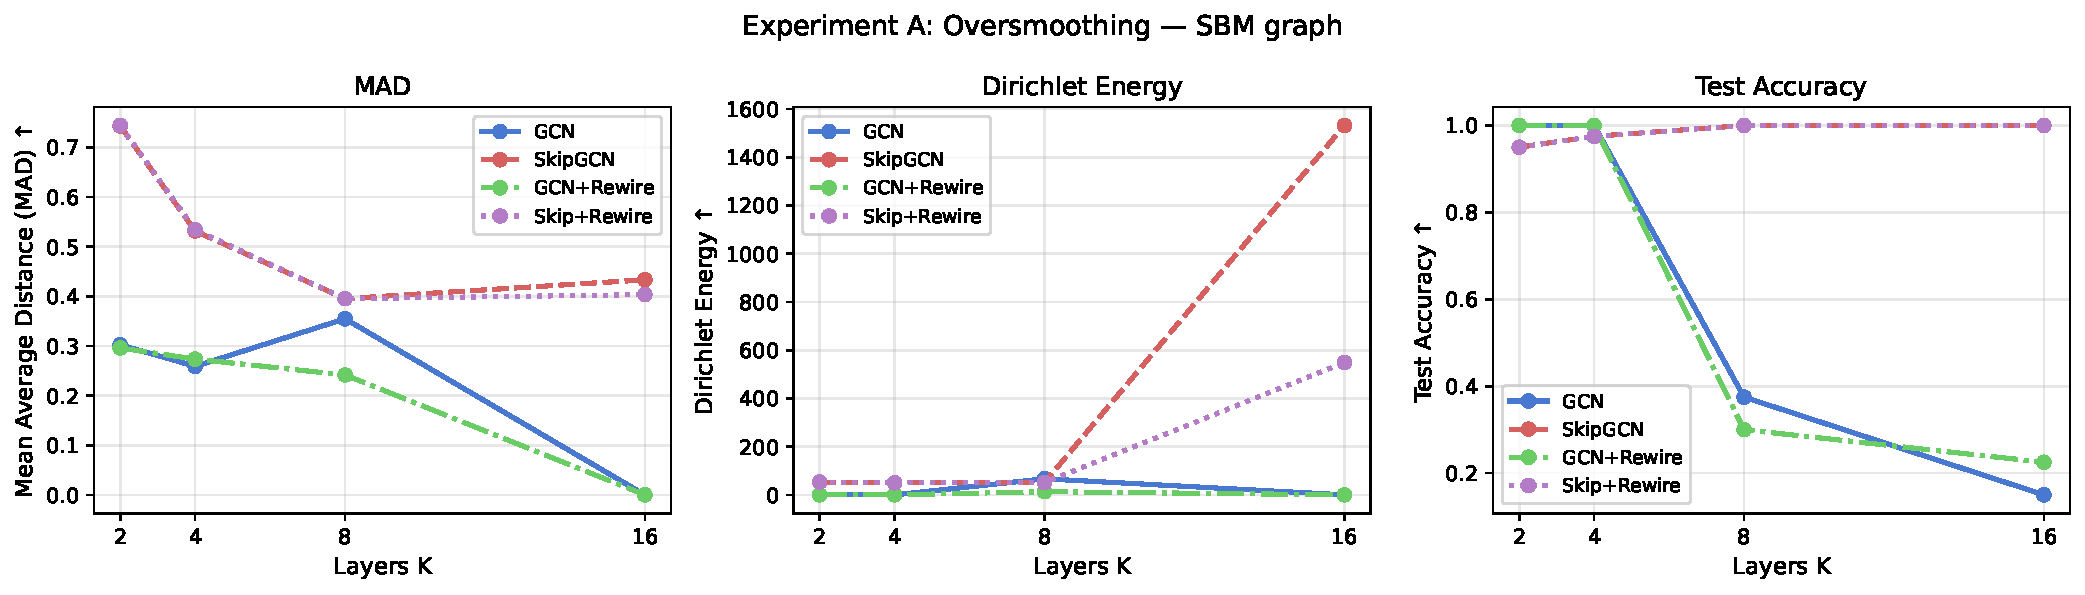
\includegraphics[width=0.98\linewidth]{exp_a_oversmoothing.pdf}
\caption{Experiment A (SBM, mean$\pm$std over 5 seeds). GCN collapses with depth
(MAD$\to0$, Acc$\to$chance); skip connections mitigate but show large variance at
$K{=}16$; rewiring lowers MAD and accuracy relative to its non-rewired counterpart.}
\label{fig:expA}
\end{figure}

\begin{figure}[t]
\centering
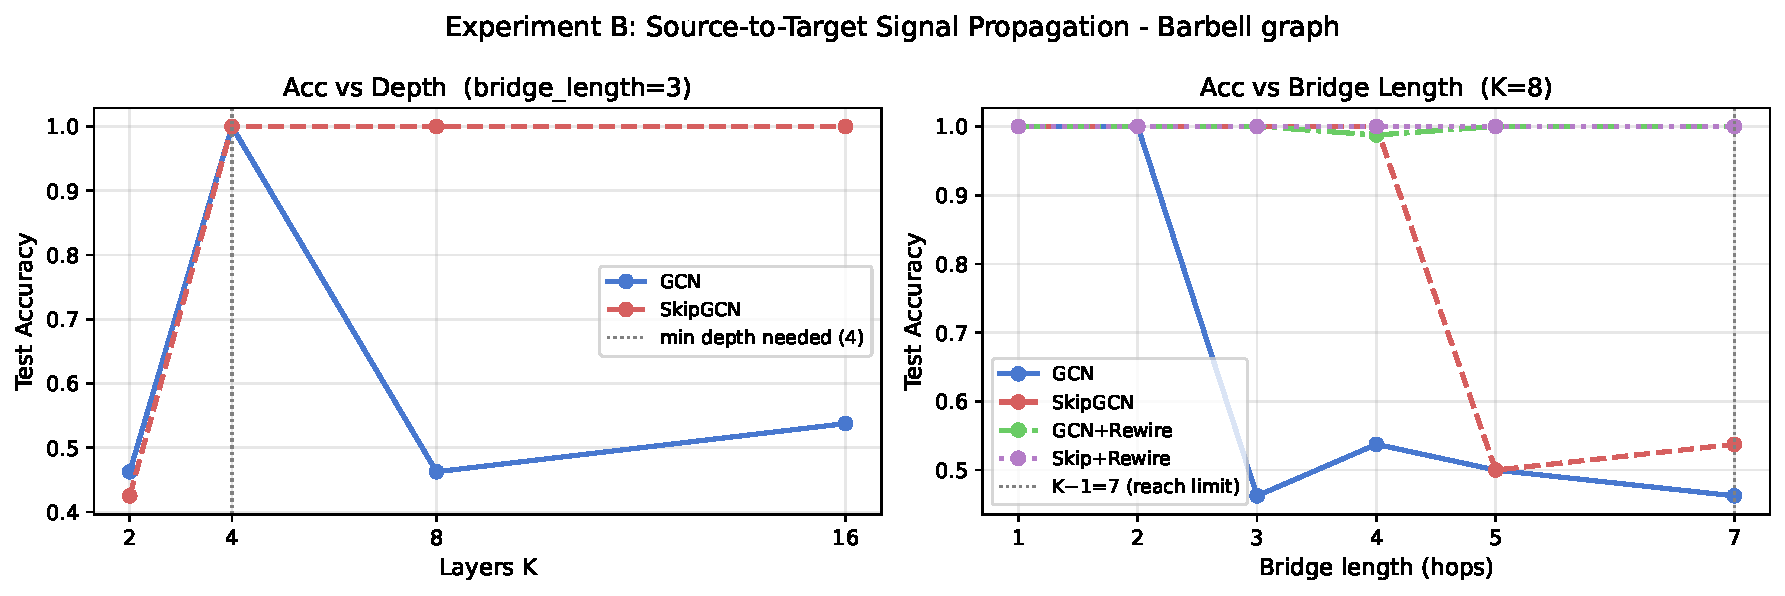
\includegraphics[width=0.98\linewidth]{exp_b_oversquashing.pdf}
\caption{Experiment B (barbell, mean$\pm$std over 5 seeds). Left: accuracy vs.\ depth
($b{=}3$). Right: accuracy vs.\ bridge length ($K{=}8$). Rewired conditions are at
$1.0$ throughout; \textsc{SkipGCN} fails for $b\ge5$.}
\label{fig:expB}
\end{figure}

\begin{table}[t]
\centering
\small
\caption{Over-squashing: target-node accuracy vs.\ bridge length ($K{=}8$,
mean$\pm$std over 5 seeds). Rewiring is invariant to bridge length; skip connections
break at $b\ge5$.}
\label{tab:bridge}
\begin{tabular}{lcccccc}
\toprule
$b$ (hops) & 1 & 2 & 3 & 4 & 5 & 7 \\
\midrule
\textsc{GCN}          & 1.00 & .90$\pm$.20 & .57$\pm$.22 & .50$\pm$.04 & .50$\pm$.02 & .49$\pm$.04 \\
\textsc{SkipGCN}      & 1.00 & 1.00 & 1.00 & .73$\pm$.23 & .46$\pm$.04 & .51$\pm$.04 \\
\textsc{GCN+Rewire}   & 1.00 & 1.00 & 1.00 & 1.00 & 1.00 & 1.00 \\
\textsc{Skip+Rewire}  & 1.00 & 1.00 & 1.00 & 1.00 & 1.00 & 1.00 \\
\bottomrule
\end{tabular}
\end{table}

\begin{table}[t]
\centering
\small
\caption{Summary at $K{=}8$ (mean$\pm$std over 5 seeds). $\uparrow$ better. MAD low
$=$ oversmoothed.}
\label{tab:summary}
\begin{tabular}{lccc}
\toprule
Model & MAD (SBM)$\uparrow$ & Acc (SBM)$\uparrow$ & Acc (Barbell $b{=}3$)$\uparrow$ \\
\midrule
\textsc{GCN}          & .329$\pm$.047 & .640$\pm$.227 & .565$\pm$.218 \\
\textsc{SkipGCN}      & .381$\pm$.040 & .965$\pm$.034 & \textbf{1.000$\pm$.000} \\
\textsc{GCN+Rewire}   & .290$\pm$.056 & .440$\pm$.147 & \textbf{1.000$\pm$.000} \\
\textsc{Skip+Rewire}  & .379$\pm$.028 & .970$\pm$.037 & \textbf{1.000$\pm$.000} \\
\bottomrule
\end{tabular}
\end{table}

\section{Discussion}
\label{sec:discussion}

\paragraph{Relation to literature and course concepts (e).}
Our oversmoothing collapse and the MAD/Dirichlet diagnostics reproduce
\cite{li2018deeper,oono2020,rusch2023survey}; the residual fix follows the
skip-connection idea from Practical~3 and jumping-knowledge networks
\cite{xu2018jk,he2016}. Our over-squashing setup operationalises the bottleneck
argument of \cite{alon2021} and the curvature view of \cite{topping2022}; the
Jacobian-vs-distance diagnostic is the sensitivity formalism of
\cite{digiovanni2023}. The novel element is the \emph{interaction}: the literature
studies each remedy against its own pathology, whereas we cross them and expose an
asymmetric trade-off rooted in a single mechanism (message averaging)---the central
theme of the course's information-propagation lectures. The result can also be read
through \emph{inductive bias}: rewiring trades a long-range bias for faster mixing.

\paragraph{Critical perspective (f).}
Several caveats temper the findings. (1) \textbf{Rewiring ``wins'' partly by
changing the task}: SDRF collapses the source--target distance to $1$--$2$ hops, so
at $K{=}8$ the problem becomes trivial---the perfect $1.000\pm.000$ reflects an
easier graph, not a model that squashes less. (2) The barbell metric is
\textbf{bimodal} (runs either solve it, $\approx1.0$, or sit at chance, $\approx0.5$);
a mean of $0.73$ means ``$3/5$ seeds solved it,'' not a typical $73\%$. (3) Skip
connections are a \emph{mitigation, not a cure}: at $K{=}16$ ($.86\pm.26$) and
$b{=}4$ ($.73\pm.23$) they are unreliable. (4) The Jacobian's absolute scale is
unstable across seeds (e.g.\ SkipGCN $5.2\pm5.2$ at distance $1$); only the decay
\emph{slope} and the order-of-magnitude gap are trustworthy. (5) Dirichlet energy is
unbounded and noisy---we rely on MAD and accuracy. (6) Exp.~A varies only
initialisation (fixed SBM), and the rewiring is SDRF-\emph{inspired}, not exact SDRF.
(7) The testbeds are small and synthetic by design; they isolate mechanisms cleanly
but do not establish magnitudes on real graphs.

\section{Conclusions and Outlook}
\label{sec:conclusion}

In a controlled $2\times2$ study we find that skip connections and curvature-based
rewiring are \emph{complementary but asymmetric}: rewiring reliably fixes
over-squashing yet worsens oversmoothing, skip connections mitigate oversmoothing
and moderate over-squashing but fail on severe bottlenecks, and only their
combination is robust on both. Practically, ``stacking fixes'' is justified here, but
each fix has a cost on the opposite axis.

\paragraph{Outlook (g).}
Stronger conclusions require: (i) real long-range benchmarks (e.g.\ LRGB
Peptides) to test whether the trade-off persists beyond synthetic graphs;
(ii) faithful SDRF (softmax-sampled by curvature gain) and alternative rewirings
(FoSR, GTR) to separate ``shortening the path'' from ``relieving curvature'';
(iii) normalisation baselines (PairNorm, GraphNorm) as a third oversmoothing remedy;
and (iv) a graph where rewiring \emph{cannot} trivially shorten the source--target
distance, to test rewiring's benefit when it does not change task difficulty.

\begin{thebibliography}{99}
\small
\bibitem{li2018deeper} Q.~Li, Z.~Han, X.-M.~Wu. Deeper insights into graph
convolutional networks for semi-supervised learning. \emph{AAAI}, 2018.
\bibitem{oono2020} K.~Oono, T.~Suzuki. Graph neural networks exponentially lose
expressive power for node classification. \emph{ICLR}, 2020.
\bibitem{rusch2023survey} T.~K.~Rusch, M.~M.~Bronstein, S.~Mishra. A survey on
oversmoothing in graph neural networks. \emph{arXiv:2303.10993}, 2023.
\bibitem{alon2021} U.~Alon, E.~Yahav. On the bottleneck of graph neural networks and
its practical implications. \emph{ICLR}, 2021.
\bibitem{topping2022} J.~Topping, F.~Di~Giovanni, B.~Chamberlain, X.~Dong,
M.~Bronstein. Understanding over-squashing and bottlenecks on graphs via curvature.
\emph{ICLR}, 2022.
\bibitem{digiovanni2023} F.~Di~Giovanni, L.~Giusti, F.~Barbero, et al. On
over-squashing in message passing neural networks: the impact of width, depth, and
topology. \emph{ICML}, 2023.
\bibitem{he2016} K.~He, X.~Zhang, S.~Ren, J.~Sun. Deep residual learning for image
recognition. \emph{CVPR}, 2016.
\bibitem{xu2018jk} K.~Xu, C.~Li, Y.~Tian, et al. Representation learning on graphs
with jumping knowledge networks. \emph{ICML}, 2018.
\bibitem{kipf2017} T.~N.~Kipf, M.~Welling. Semi-supervised classification with graph
convolutional networks. \emph{ICLR}, 2017.
\end{thebibliography}

\appendix
\section{Curvature distribution}
\label{app:curv}
\begin{figure}[h]
\centering
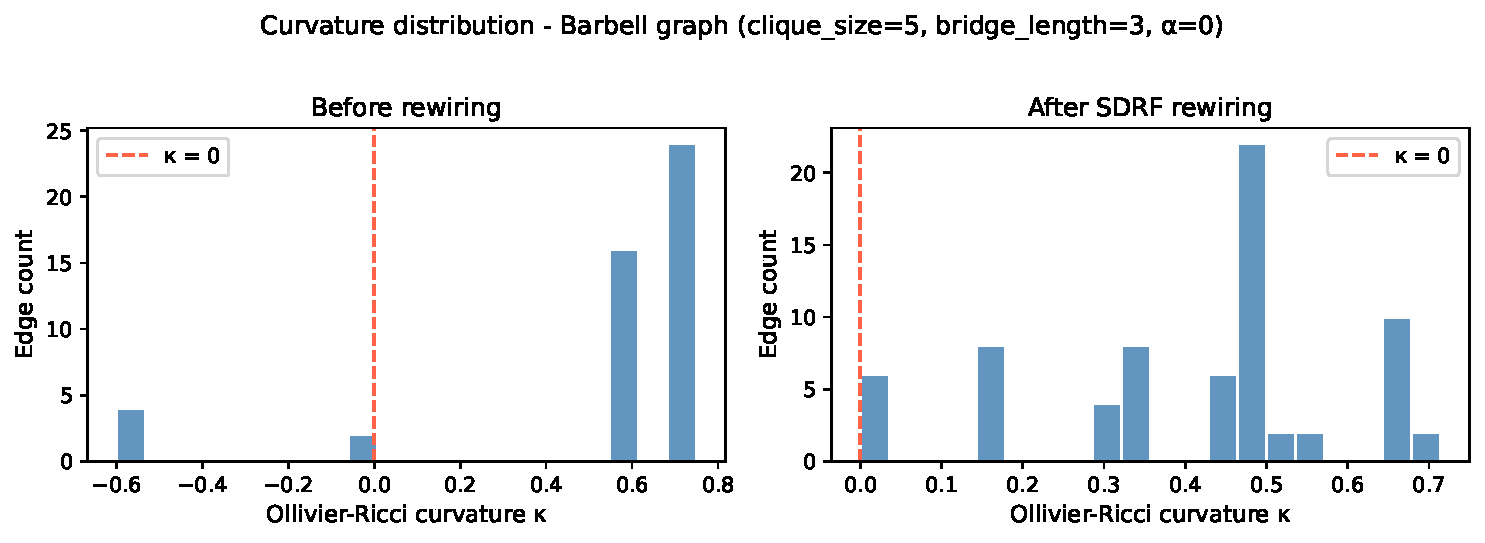
\includegraphics[width=0.86\linewidth]{curvature_distributions.pdf}
\caption{Ollivier--Ricci curvature of the barbell before/after rewiring. The negative
(bottleneck) edges are removed and the distribution shifts positive.}
\end{figure}

\end{document}
